\chapter{Spectral Relaxations of Balanced Graph Cuts}%{Spectral Methods for Video Segmentation}
\label{SpectRelax}
Spectral clustering techniques have become one of the major clustering methods over the past few years. 
The reasons are their well-understood theoretical foundation and generality. Spectral clustering can be applied to any kind of data where similarity measure is available
to build a neighbourhood graph and can be solved efficiently by standard linear algebra software. Results obtained by spectral clustering often outperform the traditional clustering approaches.
Spectral methods have proved to be successful in many video segmentation algorithms~\cite{Brox10,GalassoCS12,Galasso14}. They convince by the ability to include long-range affinities and
the globalization effect~\cite{Fowlkes04}.

In this chapter we focus on the motivation of spectral clustering based on balanced graph cut criteria. We start by presenting different balanced graph cut objectives and continue with overview of 
relaxation techniques of the NP-hard balanced cut problem. We introduce a standard 2-norm relaxation approach, which known to be loose and may lead to a solution far from the optimal one of the original problem~\cite{guattery1998},
and a tight 1-norm relaxation technique, called 1-spectral clustering~\cite{Buhler09,Hein10,HeinS11}, which in practice usually outperforms the standard loose relaxation and yields much better graph cuts.
%Further the generalization of 1-spectral clustering which integrates must-link constraints, the method called COSC~\cite{RangapuramH12}, is presented. 
%
% 
% The method, called COSC, is based on a tight relaxation of the constrained normalized cut into
% an unconstrained continuous optimization problem and is the first one, where all given constraints are fulfilled.  
% 
% Solving balanced graph cut problems is well-known
% to be NP-hard~\cite{Wagner93}. 
% 
% Spectral clustering as a graph-based approach to clustering is originally derived as a relaxation
% of the NP-hard balanced graph cut problem. 
% 
% We introduce a standard 2-norm relaxation approach, which known to be loose and may lead to a solution far from the optimal one of the original problem~\cite{guattery1998},
% and a tight 1-norm relaxation technique, called 1-spectral clustering~\cite{Buhler09,Hein10,HeinS11}. In practice it usually outperforms the standard loose relaxation and yields much better graph cuts.
% 
% leads to an eigenproblem for the graph Laplacian, where the second eigenvectors of the unnormalized and normalized graph Laplacians correspond to relaxations
% of the ratio cut~\cite{HagenK91} and normalized cut~\cite{Shi00}. However, it is often quite loose and may lead to a solution far from the optimal one of the original problem~\cite{guattery1998}.
% 
% Recently, it has been shown that all balanced graph cut problems have a tight relaxation into continuous optimization problem using the nonlinear 1-graph Laplacian~\cite{Buhler09,Hein10,HeinS11}. This tight relaxation is called 
% 1-spectral clustering. Although this technique provides no guarantee of convergence to the globally optimal solution, in practice it usually outperforms the standard loose relaxation and yields much better graph cuts.
% 
% In further work the generalization of 1-spectral clustering technique which integrates must-link constraints has been shown in~\cite{RangapuramH12}. 
% The method, called COSC, is based on a tight relaxation of the constrained normalized cut into
% an unconstrained continuous optimization problem and is the first one, where all given constraints are fulfilled.  
\section{Clustering as Graph Partitioning}
\label{sec:ch2_clgrpart}
%In this thesis to obtain the final video segmentation we consider clustering as a graph partitioning problem.
Clustering can be seen as a graph partitioning problem.
Suppose we are given a set of data points $\{x_i\}_{i=1}^n$ and some notion of similarity measure $W\colon X\times X\rightarrow \mathbb{R}$. 
The intuition behind the clustering is to group points into different sets according to their similarities. 

The data can be transformed into a weighted, undirected graph $G =(V,W)$, where the vertices $V$ of the graph represent the data points and the positive edge weights $W$ encode the similarity between pairs of points.
The matrix $W = \{w_{ij}\}_{i,j=1}^n$ is called the affinity matrix. When constructing similarity graphs the goal is to model local neighbourhood relationships between the points, to build the global structure inherent in the data 
from the local structure.

The problem of clustering can be reformulated using the similarity graph: we want to find the partition such that the edges inside the group of points have very high weights (high within-cluster similarity) and the edges between different groups of points 
have very low weights (low between-cluster similarity). A clustering of points is then equivalent to a partition of $V$ into subsets $C_1,\dots,C_k$, where $k$ is the desired number of clusters. 

Let us introduce some notions. The degree of vertex $v_i\in V$ is defined by the degree function $d\colon V\rightarrow \mathbb{R}$, $d_i = \sum_{j=1}^n w_{ij}$. The degree matrix $D$ is defined as $D_{ij} = d_i\delta_{ij}$. 
Given a subset of vertices $A\subset V$, its complement is denoted as $\overline{A} = V\backslash A$. For two not necessarily disjoint sets $A,B\subset V$ we define
\begin{equation*}
W(A,B) = \sum\limits_{i\in A, j\in B} w_{ij}.
\end{equation*}
And the cut value of $A\subset V$ and $\overline{A}$ is defined as 
%\begin{equation*}
$\mathrm{cut}(A,\overline{A}) = W(A,\overline{A})$. %\sum\limits_{i\in A, j\in \overline{A}} w_{ij}.
%\end{equation*}

Using these definitions several criteria for graph partitioning can be defined.
One way to obtain the partition of the graph is to solve the min-cut problem. For a given number of clusters $k$, the min-cut approach consists in choosing the partition  $C_1,\dots,C_k$ which minimizes
\begin{equation}
\label{eq:mincut}
\mathrm{MinCut}(C_1,\dots,C_k) = \frac{1}{2} \sum\limits_{i=1}^k \mathrm{cut}(C_i,\overline{C_i}).
\end{equation}
The min-cut problem is well researched and can be solved efficiently in polynomial time (notably the Edmonds-Karp algorithm). However, in practice solving~\eqref{eq:mincut} often leads to trivial partitions. 
The solution of min-cut may just disconnect one individual point or a few points from the set. This is not what we want to see in the clustering solution, as clusters 
should be reasonably large group of points. The way to deal with this problem is to explicitly request that the clusters should be of equal size. Therefore one has to introduce some balancing term which biases the cut criterion 
towards balanced partitions.  
In the unsupervised clustering when the focus is on pairwise terms the balancing property of graph cuts is favourable, whereas the graph partitioning techniques based on the min-cut formulation are suited for problems
with strong unary terms.
\section{Balanced Graph Cut Criteria}
\label{sec:ch2_balgrcut}
In our work we aim to investigate the influence of different balanced graph cut objectives on the final video segmentation result.
Several balanced graph cut criteria have been proposed in the literature, all of them request the size of the clusters to be ``reasonably large``.
%One way to obtain the desirable solution is to balance the size of clusters. 

There are two different approaches how to measure the size of a set in a graph. We can favour solutions which give clusters with equal cardinality $\lvert A \rvert$ 
(cardinality of set $A$) or with equal volume $\mathrm{vol}(A) = \sum_{i \in A} d_i$ (see fig.~\ref{fig:bal_cr}).
\begin{figure}[h!]
 \centering
 \subfigure[Balancing of cardinality]{%
 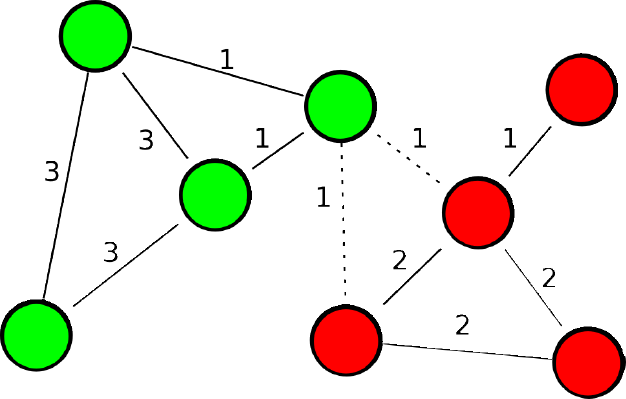
\includegraphics[width=0.4\textwidth]{images/png/card.png}
\label{fig:subfigure1}}
\quad
\qquad
 \subfigure[Balancing of volume]{%
 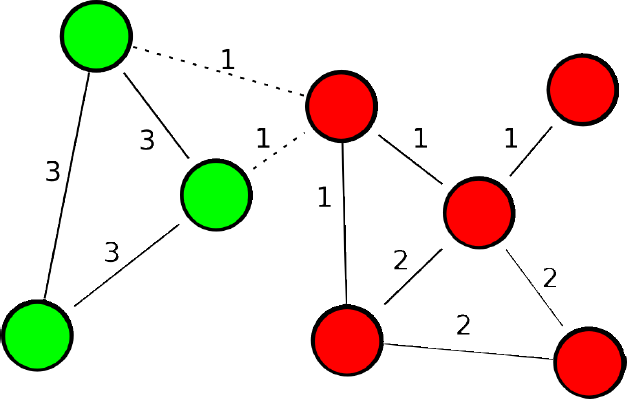
\includegraphics[width=0.4\textwidth]{images/png/vol.png}
\label{fig:subfigure2}}
 \caption[Two different ways of balancing the size of clusters]{
  {\bf Two different ways of balancing the size of clusters} (courtesy of~\cite{HeinBuh09}).}
\label{fig:bal_cr}
\end{figure}
Using these two balancing terms one can define several balanced graph cut criteria which can be used for graph partitioning. Commonly used balanced graph cut criteria are the ratio cut $\mathrm{RCut}(C,\overline{C})$~\cite{HagenK91} and 
the normalized cut $\mathrm{NCut}(C,\overline{C})$~\cite{Shi00},
which are defined as
\begin{equation}
\mathrm{RCut}(C,\overline{C}) =  \frac{\mathrm{cut}(C,\overline{C})}{\lvert C \rvert} + \frac{\mathrm{cut}(C,\overline{C})}{\lvert \overline{C} \rvert},
\end{equation}
\begin{equation}
\mathrm{NCut}(C,\overline{C}) =  \frac{\mathrm{cut}(C,\overline{C})}{\mathrm{vol}(C)} + \frac{\mathrm{cut}(C,\overline{C})}{\mathrm{vol}(\overline{C})}.
\end{equation}
Related criteria with slightly different balancing behaviour are the corresponding ratio Cheeger cut $\mathrm{RCC}(C,\overline{C})$~\cite{c70} and normalized Cheeger cut $\mathrm{NCC}(C,\overline{C})$ defined as
\begin{equation}
  \displaystyle \mathrm{RCC}(C,\overline{C}) =  \frac{\mathrm{cut}(C,\overline{C})}{\min{\{\lvert C \rvert,\lvert \overline{C} \rvert\}} }, 
\end{equation}
\begin{equation}
  \displaystyle \mathrm{NCC}(C,\overline{C}) =  \frac{\mathrm{cut}(C,\overline{C})}{\min{\{\mathrm{vol}(C),\mathrm{vol}(\overline{C})\}} }. 
\end{equation}
One has the following simple relation between the normalized cut $\mathrm{NCut}(C,\overline{C})$ and the normalized Cheeger cut $\mathrm{NCC}(C,\overline{C})$:
\begin{equation*}
 \mathrm{NCC}(C,\overline{C})\leq \mathrm{NCut}(C,\overline{C})\leq \mathrm{2NCC}(C,\overline{C}).
\end{equation*}
The same result holds for the ratio cut $\mathrm{RCut}(C,\overline{C})$ and the ratio Cheeger cut $\mathrm{RCC}(C,\overline{C})$.

Generally, clustering has two different objectives:
\begin{enumerate}
\item We want to find the partition which minimizes the between-cluster similarity. This means to minimize the cut value $\mathrm{cut}(C,\overline{C})$.
\item We want to find the partition which maximizes the within-cluster similarities $W(C,C)$ and $W(\overline{C},\overline{C})$.
\end{enumerate}

Both the ratio and the normalized cut, as well as the Cheeger cuts, directly fulfill the first objective by explicitly incorporating the value of $\mathrm{cut}(C,\overline{C})$ in the objective function. 
However, concerning the second point the algorithms behave differently due to its balancing terms. As $W(C,C)= W(C,V)-W(\overline{C},\overline{C}) = \mathrm{vol}(C)-\mathrm{cut}(C,\overline{C})$, 
the within-cluster similarity is maximized if $\mathrm{vol}(C)$ is large and the cut value is small. This is exactly
achieved by the normalized cut $\mathrm{NCut}$. In order to fulfill the second objective, another balanced graph cut criterion can be considered, namely the $\mathrm{MinMaxCut}$ criterion~\cite{DingHZGS01}:
\begin{equation}
 \mathrm{MinMaxCut}(C,\overline{C}) =  \frac{\mathrm{cut}(C,\overline{C})}{W(C,C)} + \frac{\mathrm{cut}(C,\overline{C})}{W(\overline{C},\overline{C})}.
\end{equation}
In practice, $\mathrm{NCut}$ and $\mathrm{MinMaxCut}$ are often minimized by similar partitions, as a good solution will have a small value of $\mathrm{cut}(C,\overline{C})$ and hence
their denominators are not so different. Moreover, relaxing $\mathrm{MinMaxCut}$ leads exactly to the same optimization problem as relaxing
$\mathrm{NCut}$~\cite{Luxb07}.
As for the ratio cut, here the objective is to maximize cardinality instead of volume. But the within-cluster similarity depends on the edges and not on the number of vertices in the cluster. Therefore by minimizing $\mathrm{RCut}$ the
second objective is not achieved.

For multipartition of $V$ into $k$ clusters $C_1,\dots,C_k$ the ratio, normalized cuts and the $\mathrm{MinMaxCut}$ can be generalized~\cite{Luxb07} as
\begin{equation}
\mathrm{RCut}(C_1,\dots,C_k) =  \sum \limits_{i=1}^k \frac{\mathrm{cut}(C_i,\overline{C_i})}{\lvert C_i \rvert} ,
\end{equation}
\begin{equation}
\mathrm{NCut}(C_1,\dots,C_k) =  \sum \limits_{i=1}^k \frac{\mathrm{cut}(C_i,\overline{C_i})}{\mathrm{vol}(C_i)}.
\end{equation}
\begin{equation}
 \mathrm{MinMaxCut}(C_1,\dots,C_k)) = \sum \limits_{i=1}^k \frac{\mathrm{cut}(C_i,\overline{C_i})}{W(C_i,C_i)}.
\end{equation}
The commonly recognized multipartition version of the Cheeger cuts does not exist.

% Both objective functions take a small value if clusters $C_i$ are not too small: the minima of $\sum_{i=1}^k 1\backslash{\lvert C_i \rvert}$ and $\sum_{i=1}^k 1\backslash{\mathrm{vol}(C_i)}$ are achieved if all $\lvert C_i \rvert$ and
% $\mathrm{vol}(C_i)$ coincide correspondingly.
One should also mention that balancing term only has an impact 
if the size of cardinality or volume is small, usually the cut value itself dominates what is selected for the partition. It simply helps to avoid the extreme
cases where the clusters are highly unbalanced.

We are interested in the optimal $\mathrm{RCut}$/$\mathrm{NCut}$ and search for the minimum among all possible partitions,
\begin{equation}
\label{eq:np}
\min\limits_{C_1,\dots,C_k} \mathrm{NCut}(C_1,\dots,C_k).
\end{equation}
However, introducing balancing terms makes the graph partitioning problem~\eqref{eq:np} NP-hard~\cite{Wagner93}. In practice we use spectral relaxations of this problem. 
We can write the normalized cut as
\begin{equation*}
\mathrm{NCut}(C_1,\dots,C_k) = \sum \limits_{i=1}^k \frac{\sum _{r,s=1}^n \mathds{1}_{r \in C_i} w_{ij} (1 - \mathds{1}_{s \in C_i)}}{\sum_{r=1}^n \mathds{1}_{r \in C_i} d_r},
\end{equation*}
so that finding the optimal partition can be seen as a combinatorial optimization problem. We will see below that a slightly different way of writing balanced graph cut criteria suggests a relaxation, where 
the constraints are relaxed. Thus the set of possible solutions becomes larger and the optimal value of the relaxed problem is smaller than the one of the original problem. We go from combinatorial 
to a continuous problem which is potentially easier to solve. Spectral clustering algorithms are based on this kind of relaxation.
%For this relaxation we could even find the globally optimal solution. 
\section{Spectral Clustering}
\label{sec:ch2_spectclus}
In our work we want to study the effects of the 2-norm relaxation of balanced graph cuts which leads to spectral clustering on video segmentation.
This section presents a short overview of the spectral relaxation technique, two variants of spectral clustering algorithmic schemes and argues about the quality of the solution
obtained by the standard spectral method. 

The spectral relaxation of the balanced graph cut problem results in the linear eigenproblem for the graph Laplacian~\cite{HagenK91,Shi00,Luxb07}. Therefore in order to proceed 
with the 2-norm relaxation, we first briefly recall some notions of the graph Laplacian and point out the most important properties.
%In order to proceed with relaxations of balanced graph cut problem, we first briefly recall some notions of the graph Laplacian and point out the most important properties.
\subsubsection*{Graph Laplacian}
In the following we always assume that $G$ is an 
undirected, weighted graph with affinity matrix $W$.
%\subsubsection*{The unnormalized graph Laplacian}
The unnormalized graph Laplacian is defined as 
\begin{equation*}
\Delta_{2}^{(u)} = D-W.
\end{equation*}
There are two matrices which are called normalized graph Laplacians in the literature. Since the first one is closely related to a random work on the graph, it is called normalized random walk graph Laplacian 
and the other one normalized graph Laplacian. Both of them are closely related and are defined as
\begin{equation*}
\begin{aligned}
&\Delta_{2}^{(rw)} = I-D^{-1}W,\\
&\Delta_{2}^{(n)} = I-D^{-1/2}WD^{-1/2}.
\end{aligned}
\end{equation*} 
Note that $\Delta_{2}^{(u)} = D\Delta_{2}^{(rw)}$ and $\Delta_{2}^{(n)} = D^{-1/2}\Delta_{2}^{(u)}D^{-1/2}$.

An overview over the properties of graph Laplacians can be found in~\cite{Luxb07}. The most important properties are summarized in the following proposition~\cite{HeinNotes}.
\begin{proposition}
\begin{enumerate}
\item For every vector $f\in\mathbb{R}^n$ 
\begin{equation*}
\begin{aligned}
\langle f,\Delta_{2}^{(u)}f\rangle &= \langle f,\Delta_{2}^{(rw)}f\rangle= \frac{1}{2}\sum \limits_{i,j=1}^n w_{ij} ( f_i - f_j )^2 ,\\
\langle f,\Delta_{2}^{(n)}f\rangle &= \frac{1}{2}\sum \limits_{i,j=1}^n w_{ij} ( \frac{f_i}{\sqrt{d_i}} - \frac{f_j}{\sqrt{d_j}} )^2,
\end{aligned}
\end{equation*}
where $\langle \cdot,\cdot\rangle$ denotes the inner product in $\mathbb{R}^n$.
\item All graph Laplacians are positive semi-definite and self-adjoint.
\item $\Delta_{2}^{(rw)} = I-D^{-1}W$ and $\Delta_{2}^{(n)} = I-D^{-1/2}WD^{-1/2}$ are similar, $\Delta_{2}^{(rw)} =D^{-1/2}\Delta_{2}^{(n)}D^{1/2}$.
Therefore $\Delta_{2}^{(n)}u_i = \lambda_i u_i \iff v_i = D_{-1/2}u_i,\quad\Delta_{2}^{(rw)} v_i = \lambda_i v_i$.
\item Let $A_i$, $i=1,\dots,K$ be the connected components of the graph. $\mathds{1}_{j \in A_i}$ are eigenvectors of $\Delta_{2}^{(rw)}$ and $\Delta_{2}^{(u)}$ to the eigenvalue 0.
$\sqrt{d_j} \mathds{1}_{j \in A_i}$ are eigenvectors of $\Delta_{2}^{(n)}$ to the eigenvalue 0.
\item The eigenvectors of $\Delta_{2}^{(u)}$ and $\Delta_{2}^{(n)}$ define an orthonormal basis on $\mathbb{R}^V$.
\end{enumerate}
\end{proposition}
% 
% The associated regularization functionals with the graph Laplacian are:

The following properties motivate the use of eigenvectors of the graph Laplacian for finding the best partition of the graph. Later we will see that the minimum and minimizer of the relaxed balanced graph cut problem are exactly 
the second eigenvalue and second eigenvector of the graph Laplacian, which leads to the formulation of spectral clustering - the relaxation of the balanced graph cut criteria problem.   
\subsubsection*{Relaxation of Balanced Graph Cuts for Laplacian}%{Approximating $RCut$ and $NCut$}
For simplicity we start with the case of $\mathrm{RCut}$ and $k=2$. Our goal is to solve the following optimization problem
\begin{equation}
\label{eq:minrcut}
\min\limits_{C \in V} \mathrm{RCut}(C,\overline{C}).
\end{equation} 
\begin{lemma}
\label{lem:rcut}
Given a partition of $V$ into $C$ and $\overline{C}$ define,
\begin{equation}
\label{eq:frcut}
 f_i = \begin{cases} 
                      \sqrt{\frac{\lvert \overline{C} \rvert}{\lvert C \rvert}}   & \quad i \in C, \\
                      - \sqrt{\frac{\lvert C \rvert}{\lvert \overline{C} \rvert}} & \quad i \in \overline{C}.
                     \end{cases}
\end{equation}
Then 
\begin{equation*}
\mathrm{RCut}(C,\overline{C}) = \{\langle f, \Delta_{2}^{(u)} f \rangle\ |\langle f, \mathds{1} \rangle=0, \lVert f \rVert = \sqrt{n}, \text{ $f$  has form as in Eq.~\eqref{eq:frcut}} \}.
\end{equation*}
\end{lemma}
The proof can be found in~\cite{Luxb07}. 
Now the $\mathrm{RCut}$ objective function is conveniently rewritten using the unnormalized graph Laplacian. With the formulation of the lemma~\eqref{lem:rcut} we deal with a discrete optimization problem~\eqref{eq:minrcut} and 
it is still NP-hard.
However, now there exists a direct relaxation. Instead of allowing for $f$ to take only two possible values, we relax the problem by discarding the discreteness condition and allowing $f$ to take arbitrary values in $\mathbb{R}^V$. 
This leads to the relaxed optimization problem
\begin{equation}
\label{eq:rel}
\min \limits_{f \in \mathbb{R}^V} \{\langle f, \Delta_{2}^{(u)} f \rangle\ |\langle f, \mathds{1} \rangle=0, \lVert f \rVert = \sqrt{n}\}.
\end{equation}
By the Rayleigh-Ritz principle it can be seen that the solution of~\eqref{eq:rel} is just the second smallest eigenvalue $\lambda_2$ of $\Delta_{2}^{(u)}$. However, we are more interested
in the minimizer, which is just the second eigenvector $u_2$ of $\Delta_{2}^{(u)}$. The remaining step is to transform the eigenvector $u_2$ into a partition of the graph. There are two ways~\cite{HeinNotes}:
\begin{itemize}
\item thresholding: one defines for $t\geq 0$ the set $C_t = \{j \in V | u_2(j) > t\}$ and finds the threshold $t$ by optimizing the ratio cut criterion
\begin{equation*}
t^* = \min\limits_{t\geq 0} \mathrm{RCut}(C,\overline{C}).
\end{equation*}   
And return $C_{t^*}$ and $\overline{C}_{t^*}$ as clusters. This transformation of the second eigenvector into a graph partition provides upper and lower bounds in terms of the optimal cut~\cite{Buhler09}. 
\item k-means: one assumes that the eigenvector is basically constant on the cluster $C$ and $\overline{C}$. Under this condition k-means will give a partition similar to the one obtained by thresholding. However, for two clusters
thresholding should be preferred. k-means should only be used for more than two clusters.
\end{itemize}
Note, as long as the clusters are well-separated, the eigenvectors represent the structure well, so thresholding and k-means should provide almost the same clustering.
The same relaxation technique can be applied to the normalized cut criterion.
\begin{lemma}
\label{lem:ncut}
Given a partition of $V$ into $C$ and $\overline{C}$ define,
\begin{equation}
\label{eq:fncut}
 f_i = \begin{cases} 
                      \sqrt{\frac{\mathrm{vol}(\overline{C})}{\mathrm{vol}(C)}}   & \quad i \in C, \\
                      - \sqrt{\frac{\mathrm{vol}(C)}{\mathrm{vol}(\overline{C})}} & \quad i \in \overline{C}.
                     \end{cases}
\end{equation}
Then 
\begin{equation*}
\mathrm{\mathrm{NCut}}(C,\overline{C}) = \{\langle f, \Delta_{2}^{(u)} f \rangle\ |\langle Df, \mathds{1} \rangle=0, \langle f, Df \rangle = \mathrm{vol}(V) =\sqrt{n}, \text{ $f$ has form as in Eq.~\eqref{eq:fncut}} \}.
\end{equation*}
\end{lemma}
The proof can be found in~\cite{Luxb07}. 
Again we relaxing the problem by allowing $f$ to take arbitrary real values:
\begin{equation}
\min \limits_{f \in \mathbb{R}^V} \{\langle f, \Delta_{2}^{(u)} f \rangle\ | \langle Df, \mathds{1} \rangle=0, \langle f, Df \rangle = \mathrm{vol}(V)\}.
\end{equation}
Now by substituting $g = D^{1/2}f$ we obtain
\begin{equation}
\label{eq:minncut}
\min \limits_{g \in \mathbb{R}^V} \{\langle g, \Delta_{2}^{(n)} g \rangle\ |\langle g, D^{1/2}\mathds{1} \rangle=0, \lVert g \rVert^2 = \mathrm{vol}(V)\}.
\end{equation}
Observe that $\Delta_{2}^{(n)} = D^{-1/2} \Delta_{2}^{(u)} D^{1/2}$, $D^{1/2}\mathds{1}$ is the first eigenvector of $\Delta_{2}^{(n)}$ and $\mathrm{vol}(V)$ is a constant. 
Hence,~\eqref{eq:minncut} is in the form of the Rayleigh-Ritz principle,
and its solution $g$ is given by the second eigenvector of $\Delta_{2}^{(n)}$. By re-substituting $f = D^{-1/2}g$ we see that $f$ is the second eigenvector of the generalized eigenproblem $\Delta_{2}^{(u)}u= \lambda Du$.  
Until now, we have shown relaxations of different balanced graph cut criteria for only two clusters. This principle is also used to motivate the use of higher-order eigenvectors of the graph 
Laplacian for finding graph partitions.
The relaxation of the $\mathrm{RCut}$ and $\mathrm{NCut}$ minimization problem in the case of general number of clusters $k$ can be done in the similar way.
\begin{lemma}
\label{lem:multircut}
Given a partition of $V$ into $C_1,\dots,C_k$ define,
\begin{equation}
\label{eq:fmultircut}
\text{for $i = 1,\dots,k$ and $j=1,\dots,n$, }
 h_i(j) = \begin{cases} 
                      \sqrt{1}{\sqrt{\rvert C_i\lvert}}   & \quad j \in C_i, \\
                      0 & \quad j \in \overline{C_i}.
                     \end{cases}
\end{equation}
Then the general ratio cut can be written as
\begin{equation*}
\mathrm{RCut}(C_1,\dots,C_k) = \{Tr(H\Delta_{2}^{(u)}H^T) |HH^T = \mathds{1}_k\}.
\end{equation*}
\end{lemma}
Similar to above we relax the problem by allowing the entries of matrix $H$ to take arbitrary real values. Then the relaxed problem becomes:
\begin{equation}
\min\limits_{H \in \mathbb{R}^{n\times k}} \{Tr(H\Delta_{2}^{(u)}H^T) |HH^T = \mathds{1}_k\}.
\end{equation}
This is the standard form of a trace minimization problem, and again some version of the Rayleigh-Ritz principle tells us that the solution is given by choosing $H$ as the matrix which contains the first $k$ eigenvectors of 
$\Delta_{2}^{(u)}$ as columns. This leads to the general unnormalized spectral clustering algorithm.

For the case of finding more than two clusters for normalized cut:
\begin{lemma}
\label{lem:multincut}
Given a partition of $V$ into $C_1,\dots,C_k$ define,
\begin{equation}
\label{eq:fmultincut}
\text{for $i = 1,\dots,k$ and $j=1,\dots,n$, }
 h_i(j) = \begin{cases} 
                      \sqrt{1}{\sqrt{\mathrm{vol}(C_i)}}   & \quad j \in C_i, \\
                      0 & \quad j \in \overline{C_i}.
                     \end{cases}
\end{equation}
Then the general normalized cut can be written as
\begin{equation*}
\mathrm{NCut}(C_1,\dots,C_k) = \{Tr(H\Delta_{2}^{(u)}H^T) |HDH^T = \mathds{1}_k\}.
\end{equation*}
\end{lemma}
Relaxing the discreteness condition and substituting $T = D^{1/2}H$ we obtain the relaxed problem
\begin{equation}
\label{eq:mint}
\min\limits_{T \in \mathbb{R}^{n\times k}} \{Tr(T\Delta_{2}^{(n)}T^T) |TT^T = \mathds{1}_k\}.
\end{equation}
Again~\eqref{eq:mint} is solved by the matrix $T$ which contains the first $k$ eigenvectors of $\Delta_{2}^{(n)}$ as columns. Re-substituting $H = D^{-1/2}T$ the solution of $H$ consists of the first $k$ generalized eigenvectors
of $\Delta_{2}^{(u)}u= \lambda Du$. This yields the normalized spectral clustering.
The proof for the ratio and normalized cuts can be found in~\cite{Luxb07}. 
Note, that we still need to transform the set of eigenvectors into a partitioning of $V$. This is where k-means is usually applied.
\subsubsection*{Spectral Clustering Algorithms}
There are two variants of spectral clustering~\cite{HeinNotes}. The main difference is how the eigenvectors of the graph Laplacian are used in order to construct the graph partitioning.

The first variant of spectral clustering uses the eigenvectors to construct a new representation of the data. In this new representation one applies the standard k-means clustering. The data is assumed to be quite well clustered 
so that k-means yields reasonable results. The advantage of this approach is that it aggregates all information about the k eigenvectors. 
The disadvantage is that k-means prefers blob-like clusters which is not always the case for the embedded clusters.

The general scheme of spectral clustering is given below in Algorithm~\ref{alg:SCv1}.
\incmargin{1em}
\begin{algorithm}[hbtp]
\caption{Spectral Clustering - Variant 1}
\label{alg:SCv1}
\dontprintsemicolon
\BlankLine
\Indm  
\KwIn{affinity matrix $W$, number $k$ of clusters to construct, choice of the graph Laplacian (normalized, unnormalized).}
\Setnlsty{textbf}{}{:}
\Indp
\BlankLine
compute the graph Laplacian;\\
compute the first $k$ eigenvectors $\{ u_i \}_{i=1}^k$ (each eigenvector is normalized, $\lVert u_i\rVert=1$, $i=1,\dots,k$);\\
construct the Laplacian eigenmap by embedding $\phi: V\rightarrow \mathbb{R}^k$, $i\rightarrow z_i =(u_1(i),\dots,u_k(i))$;\\
cluster the points $\{z_i\}_{i=1}^n$ by k-means into clusters $C_1,\dots,C_k$.
\BlankLine
\Indm  
\KwOut{Clusters $C_1,\dots,C_k$.} 
\end{algorithm}
\decmargin{1em}

The alternative method is to use a sequential splitting procedure with thresholding to get more than two clusters. The outline of this method is listed in Algorithm~\ref{alg:SCv2}.
\incmargin{1em}
%\linesnumberedhidden
\begin{algorithm} [hbtp]
\caption{Spectral Clustering - Variant 2}
\label{alg:SCv2}
\dontprintsemicolon
\BlankLine
\Indm  
\KwIn{affinity matrix $W$, number $k$ of clusters to construct, choice of the graph Laplacian (normalized, unnormalized).}
\Setnlsty{textbf}{}{:}
\Indp
\BlankLine
%\showln
initialization: cluster $C_1 = V$, number of clusters $s=1$;\\
%\showln
\Repeat{
%\showln
number of clusters $s=k$}
{
build on each element of the current partition $C_i$ the graph Laplacian;\;
compute the second eigenvector on each partition;\;
compute the optimal threshold for dividing each cluster $C_i$;\;
choose to split the cluster $C_i$ so that the total multipartition cut criterion is minimized;\;
$s\Longleftarrow s+1$.
}
\BlankLine
\Indm  
\KwOut{Clusters $C_1,\dots,C_k$.} 
\end{algorithm}
\decmargin{1em}

There is still an open question how good is the partition obtained by the spectral relaxation. The answer to this is the isoperimetric inequality~\cite{Chung:1997}, which provides upper and lower bounds on the ratio and normalized
Cheeger cuts in terms of the second eigenvalue of the graph Laplacian. The optimal ratio and normalized Cheeger cuts values are defined as
\begin{equation*}
h_{\mathrm{RCC}} = \inf_{C} \mathrm{RCC}(C,\overline{C}), \quad h_{\mathrm{NCC}} = \inf_{C} \mathrm{NCC}(C,\overline{C}).
\end{equation*}
The standard isoperimetric inequality is given as
\begin{equation}
 \frac{h_{\mathrm{NCC}}^2}{2} \leq \lambda_{2} \leq  2 h_{\mathrm{NCC}},
\end{equation}
where $\lambda_2$ is the second eigenvalue of the normalized graph Laplacian. Note, while the second eigenvector of the graph Laplacian can be efficiently computed, this spectral relaxation is known to be 
loose %far from being tight
and provides non-optimal result.
\section{1-Spectral Clustering}
\label{sec:ch2_1spectclus}
In the recent line of work~\cite{Buhler09,Hein10,HeinS11} it has been shown that a tight relaxation of the balanced graph cuts exists and can be achieved by moving from linear eigenproblem to a nonlinear eigenproblem associated 
to the nonlinear graph p-Laplacian. This tight relaxation is called 1-spectral clustering. 
In this thesis we would like to adopt the 1-norm relaxation to video segmentation and study the relevance of this technique for video processing in comparison with the standard spectral clustering. 

In order to proceed with introduction to 1-spectral clustering, we first briefly recall the graph p-Laplacian and point out the most important properties.
\subsubsection*{Graph p-Laplacian}
The standard graph Laplacian induces the quadratic form, but there exists a nonlinear generalization of the graph Laplacian $\Delta_{p}$, called graph p-Laplacian~\cite{Amghibech03}
\begin{equation*}
\langle f,\Delta_{p} f\rangle = \frac{1}{2} \sum \limits_{i,j=1}^n w_{ij} \rvert f_i - f_j\rvert^p. 
\end{equation*}
Similar to the graph Laplacian we can define the unnormalized and normalized p-Laplacian $\Delta_{p}^{(u)}$ and $\Delta_{p}^{(n)}$. Let $i \in V$, then
\begin{equation*}
\begin{aligned}
(\Delta_{p}^{(u)}f)_i &= \sum \limits_{j\in V} w_{ij}\phi_p ( f_i - f_j ),\\
(\Delta_{p}^{(n)}f)_i &= \frac{1}{d_i}\sum \limits_{j\in V} w_{ij}\phi_p ( f_i - f_j ),
\end{aligned} 
\end{equation*}
where $\phi_p:\mathbb{R}\longrightarrow \mathbb{R}$ is defined for $x \in \mathbb{R}$ as
\begin{equation*}
 \phi_p(x) = \rvert x \lvert^{p-1} \sign(x).
\end{equation*}
Note, that for $p=2$ the standard graph Laplacian is recovered. As shown in~\cite{Buhler09}, one can obtain the eigenvalues of the %unnormalized 
p-Laplacian $\Delta_{p}^{(u)}$ as local minima of the functional
$F_p: \mathbb{R}^V\longrightarrow \mathbb{R}$,
\begin{equation*}
 F_p(f) = \frac{\langle f, \Delta_{p}f\rangle}{\lVert f\rVert_p^p} = \frac{1}{2} \frac{ \sum \limits_{i,j=1}^n w_{ij} \rvert f_i - f_j\rvert^p}{\lVert f\rVert_p^p}. 
\end{equation*}
\begin{theorem}
The functional $F_p$ has a critical point at $v \in \mathbb{R}^V$ if and only if $v$ is a p-eigenvector of $\Delta_{p}$. The corresponding eigenvalue $\lambda_p$ is given as $\lambda_p = F_p(v)$.
\end{theorem}
Similar to the standard case we need at least the second eigenvector to construct the partition. To obtain the second eigenvalue, we consider the functional $F_p^{(2)}: \mathbb{R}^V\longrightarrow \mathbb{R}$,
\begin{equation*}
 F_p^{(2)}(f) = \frac{\langle f, \Delta_{p}f\rangle}{\min\limits_{c \in \mathbb{R}}\lVert f-c\mathds{1}\rVert_p^p} = \frac{1}{2} \frac{ \sum \limits_{i,j=1}^n w_{ij} \rvert f_i - f_j\rvert^p}{\min\limits_{c \in \mathbb{R}}\lVert f-c\mathds{1}\rVert_p^p}. 
\end{equation*}
\begin{theorem}
The second eigenvalue $\lambda_p^{(2)}$ of the graph p-Laplacian $\Delta_{p}$ is equal to the global minimum of the functional $F_p^{(2)}$. The corresponding eigenvector $v_p^{(2)}$ can be computed using the global minimizer of $F_p^{(2)}$.
\end{theorem}
Proof can be found in~\cite{Buhler09}.
\subsubsection*{Relaxation of Balanced Graph Cuts for p-Laplacian}
The second eigenvector $v_p^{(2)}$ of the p-Laplacian can also be seen as the relaxation of balanced graph cuts~\cite{Buhler09}. For $p>1$ the second eigenvalue $\lambda_p^{(2)}$ is the solution of the relaxation problem
\begin{equation*}
 \min_{C\subset V} \mathrm{cut}(C, \overline{C}) \biggr\rvert \frac{1}{\rvert C\lvert^{\frac{1}{p-1}}} + \frac{1}{\rvert \overline{C}\lvert^{\frac{1}{p-1}}}\biggl\lvert^{p-1}.
\end{equation*}
With the special cases, 
\begin{equation*}
 \begin{aligned}
  p=2, \quad \min_{C\subset V} \mathrm{RCut}(C, \overline{C}),\\
  p\rightarrow 1, \quad \min_{C\subset V} \mathrm{RCC}(C, \overline{C}).
 \end{aligned}
\end{equation*}
In order to obtain the partitioning of the graph we use the standard procedure and threshold the second eigenvector $v_p^{(2)}$.  The optimal threshold is determined by minimizing the corresponding Cheeger cut.
For the unnormalized graph p-Laplacian $\Delta_{p}^{(u)}$ we determine 
\begin{equation}
 h_{\mathrm{RCC}}^* = \min_{C_t = \{i \in V | v_p^{(2)}(i) > t\}} \mathrm{RCC}(C_t, \overline{C}_t),
\end{equation}
and similarly for the normalized graph p-Laplacian $\Delta_{p}^{(n)}$ 
\begin{equation}
 h_{\mathrm{NCC}}^* = \min_{C_t = \{i \in V | v_p^{(2)}(i) > t\}} \mathrm{NCC}(C_t, \overline{C}_t).
\end{equation}
The question is how good the cut values obtained by thresholding the second eigenvector of the p-Laplacian compared to optimal Cheeger cuts. There are extensions of isoperimetric inequalities for $p>1$ for the normalized 
p-Laplacian~\cite{Amghibech03}
\begin{equation*}
 2^{p-1} \biggr ( \frac{h_{\mathrm{NCC}}}{p} \biggl )^p \leq \lambda_p^{(2)} \leq 2^{p-1} h_{\mathrm{NCC}},
\end{equation*}
 and for the unnormalized p-Laplacian~\cite{Buhler09}
 \begin{equation*}
 \biggr (\frac{2}{\max_i d_i} \biggl)^{p-1} \biggr ( \frac{h_{\mathrm{RCC}}}{p} \biggl)^p \leq \lambda_p^{(2)} \leq 2^{p-1} h_{\mathrm{RCC}}.
 \end{equation*}
It has been shown in~\cite{Buhler09}, that for $p>1$ 
\begin{equation}
\label{eq:ineq}
 \begin{aligned}
  h_{\mathrm{RCC}} &\leq h_{\mathrm{RCC}}^* \leq p(\max_{i \in V} d_i)^{\frac{p-1}{p}} (h_{\mathrm{RCC}})^{\frac{1}{p}},\\
  h_{\mathrm{NCC}} &\leq h_{\mathrm{NCC}}^* \leq p( h_{\mathrm{NCC}})^{\frac{1}{p}}.
 \end{aligned}
\end{equation}
When considering the limit $p\rightarrow 1$, one can observe that the upper bound for both inequalities~\eqref{eq:ineq} gets tight, which means that the cut obtained by thresholding the second eigenvalue of the p-Laplacian converges to 
the optimal Cheeger cut. 
\subsubsection*{1-Spectral Clustering Algorithm}
To obtain the desired partition into $k$ clusters one uses the sequential splitting with thresholding of the second eigenvector of the p-Laplacian. Applying k-means in this setting is not possible, since at the moment 
we are not able to compute higher-order eigenvectors of the p-Laplacian. 

The algorithmic scheme for 1-spectral clustering is presented below.
\incmargin{1em}
%\linesnumberedhidden
\begin{algorithm}[hbtp]
\caption{1-Spectral Clustering}
\label{SCv1}
\dontprintsemicolon
\BlankLine
\Indm  
\KwIn{affinity matrix $W$, number $k$ of clusters to construct, choice of the graph 1-Laplacian (normalized, unnormalized).}
\Setnlsty{textbf}{}{:}
\Indp
\BlankLine
%\showln
initialization: cluster $C_1 = V$, number of clusters $s=1$;\\
%\showln
\Repeat{
%\showln
number of clusters $s=k$}
{
minimize $F_p^{(2)}: \mathbb{R}^{C_i}\longrightarrow \mathbb{R}$ for the chosen p-Laplacian for each cluster $C_i$, $i=1,\dots,s$;\;
compute the optimal threshold for dividing each cluster $C_i$;\;
choose to split the cluster $C_i$ so that the total multipartition cut criterion is minimized;\;
$s\Longleftarrow s+1$.
}
\BlankLine
\Indm  
\KwOut{Clusters $C_1,\dots,C_k$.} 
\end{algorithm}
\decmargin{1em}
\newpage

The functional $F_p^{(2)}$ is non-convex and thus we cannot guarantee to reach the global minimum. Although a direct minimization for small values of $p$ leads often to very fast convergence to a non-optimal local minimum.
Empirical observations show that the cut found by 1-spectral clustering is always at least as good as the cut found by standard spectral clustering - often much better (see fig.~\ref{fig:1sc_sc_fig}).
\begin{figure}[htbp]
 \centering
 \subfigure[A simple graph in two dimensions]{%
 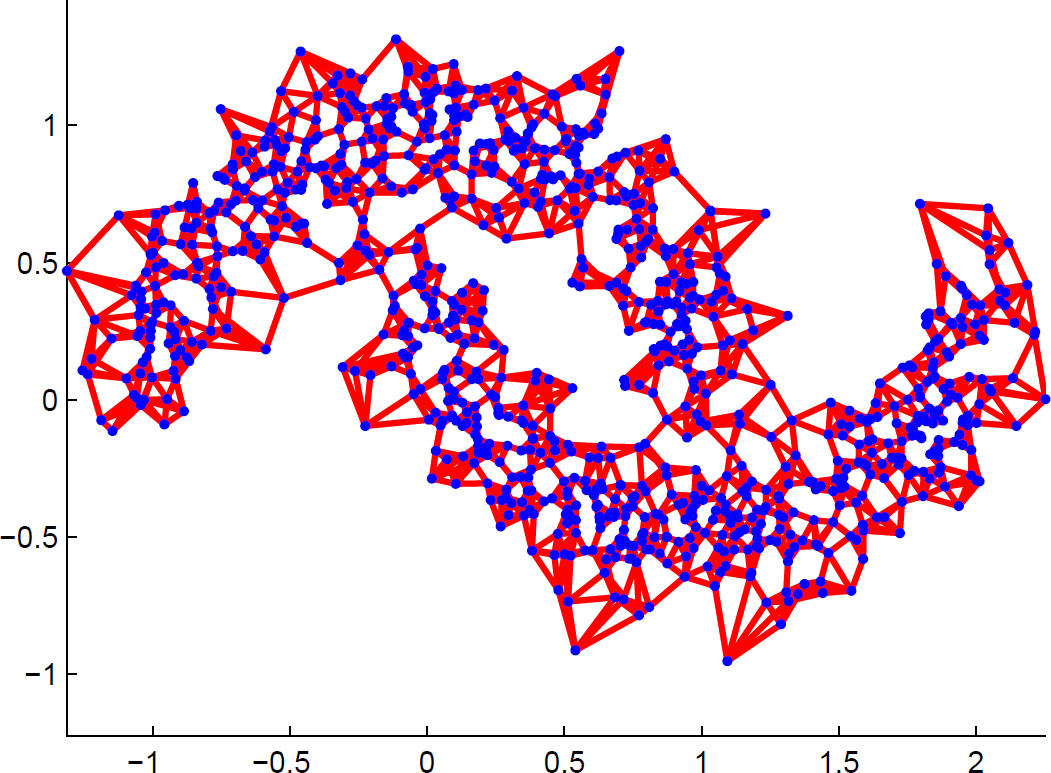
\includegraphics[width=0.32\textwidth]{images/png/sc_vs_1sc_1.png}
\label{fig:subfigure1}}
\qquad
 \subfigure[Eigenvector of the graph Laplacian]{%
 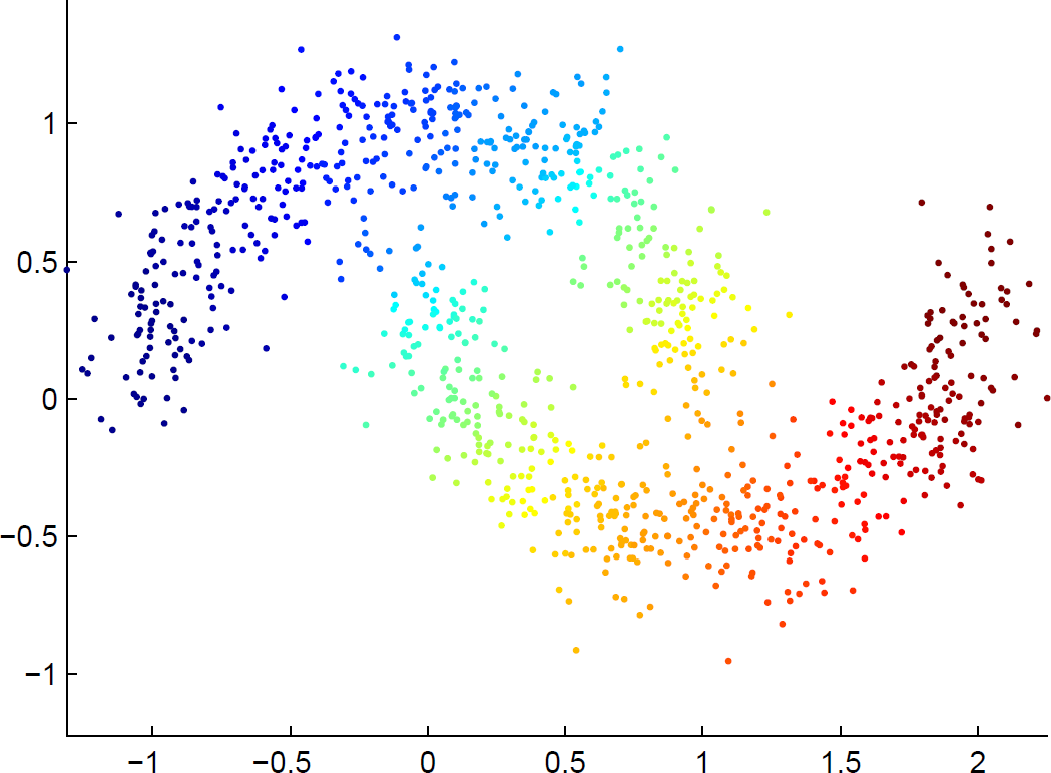
\includegraphics[width=0.32\textwidth]{images/png/sc_vs_1sc_2.png}
\label{fig:subfigure2}}
\qquad
\subfigure[Partition obtained by thresholding the second eigenvector of the graph Laplacian]{%
 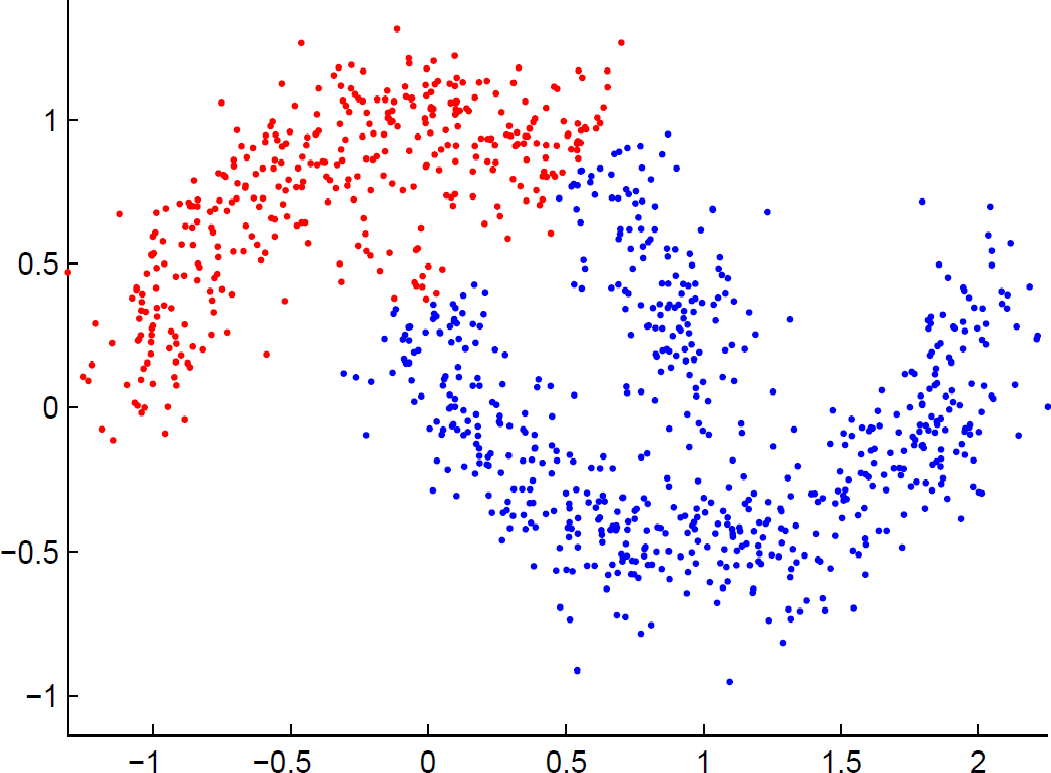
\includegraphics[width=0.32\textwidth]{images/png/sc_vs_1sc_3.png}
\label{fig:subfigure1}}
\qquad
 \subfigure[Eigenvector of the graph 1-Laplacian]{%
 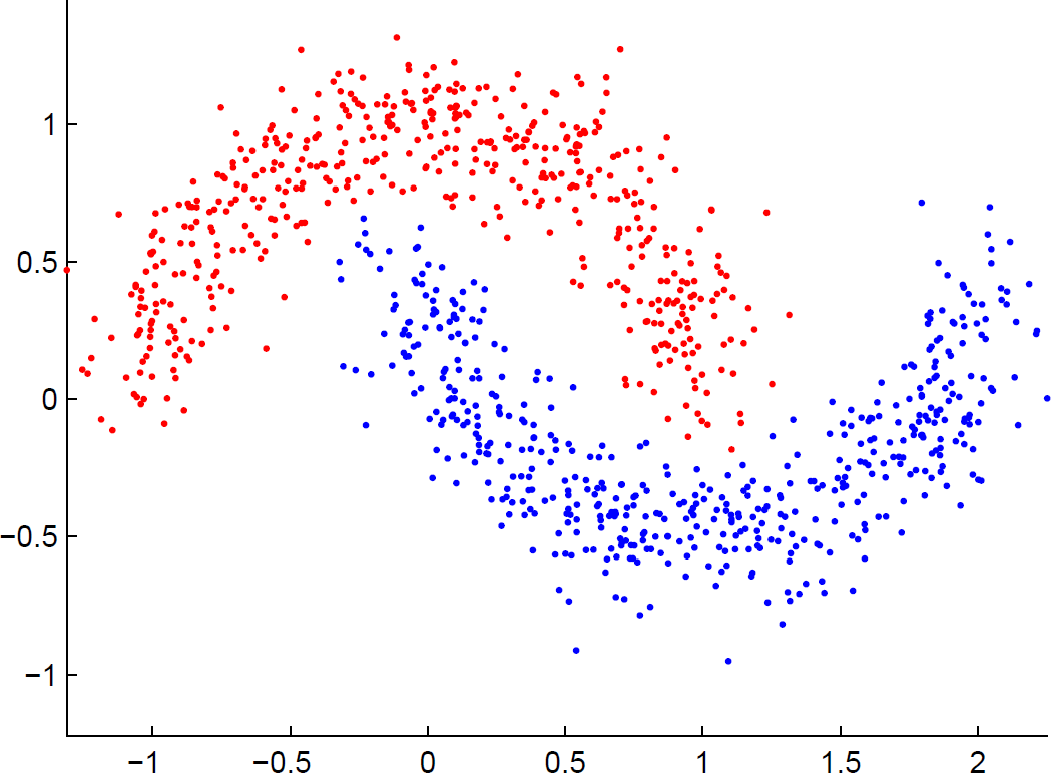
\includegraphics[width=0.32\textwidth]{images/png/sc_vs_1sc_4.png}
\label{fig:subfigure2}}
 \caption[1-spectral clustering versus standard spectral clustering]{
  {\bf 1-Spectral Clustering vs. Spectral Clustering} (courtesy of~\cite{Setzer12}).}
\label{fig:1sc_sc_fig}
\end{figure}
\sloppy
  
In further work it was shown by~\cite{Hein10} that 1-spectral clustering can be naturally formulated as nonlinear eigenproblem and the inverse power method can be applied to compute the eigenvectors of the 1-Laplacian. 
The method is guaranteed to converge to a non-constant eigenvector of the 1-Laplacian. However, the convergence to the second eigenvector is not guaranteed. Thus it is recommended to use multiple random initializations and 
use the result which achieves the best cut value.

In~\cite{HeinS11} the generalization of the spectral relaxation for almost any balanced graph cut criterion was proposed. A characterization of all balanced graph cuts has been provided, which allows a tight relaxation into 
continuous problem. Although the resulting optimization problem is non-convex and non-smooth, it can be efficiently solved by the method for the minimization of ratios of differences of convex functions, called RatioDCA. 
\section{Discussion}
\label{ch2:disc}
In this chapter we motivated spectral clustering as a relaxation of a NP-hard balanced graph cut problem and presented two relaxation methods with different graph cut objectives.

The standard 2-norm relaxation leads to a linear eigenproblem for the graph Laplacian, where the second eigenvectors
of the unnormalized and normalized graph Laplacians correspond to relaxations of the ratio cut and normalized cut. 
This spectral relaxation is known to be loose and may lead to a solution far from the optimal one of the original problem.
However, there exists a tight relaxation of a balanced graph cut problem using the nonlinear 1-graph Laplacian, called 1-spectral clustering.
This generalized non-linear eigenproblem in practice provides much better graph cuts. 
In contrast to spectral clustering, 1-spectral clustering employs a recursive splitting scheme for multipartitioning instead of a multiway approach. The reason for this is
that the computation of higher-order eigenvectors of the graph 1-Laplacian is not feasible at present.

Many successful video segmentation algorithms are based on the spectral relaxation techniques. 
But despite of all the achieved progress, adaptation of spectral clustering to video processing requires further researching.
Little attention has been paid to the effects of the 2-norm relaxation 
with different cut criteria applied to video segmentation and the tight 1-norm relaxation has not been yet adopted to video processing. 
In this thesis we aim to study the relevance of these methods for video segmentation.